\chapter{Filters}

\label{filters}
Signal filters are one of the basic tools to shape your sound in subtractive synthesis. While the oscillators in Odin 2 are already capable of a wide array of sounds, unprocessed oscillators usually sound very sharp and not pleasing to the ears. So what is a filter? A filter selectively removes frequencies from the spectrum, usually with some dials for the user to control the roll-off. Filters can be characterized by their frequency response, which tells us which frequencies are being attenuated or boosted:

\vspace{5mm}
\begin{center}
    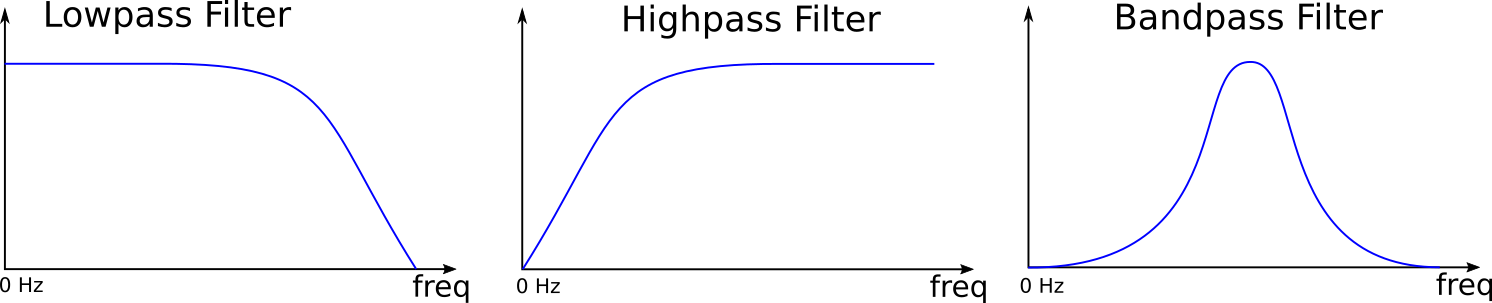
\includegraphics[width=\textwidth]{graphics/filter.png}
\end{center}

\vspace{5mm}

Odin 2 has three slots for filters which can be filled with a extensive selection of modules to shape your sound. A wide array of high quality virtual analog filter emulations is available, which emulate various analog filter circuits from synthesizer history.

TODO poly vs stereo.

\audioparameter{Filter Type}{0}{0}{To change the filter module, use the dropdown to the top-right of the filter module:

    \vspace{5mm}
    \begin{center}
        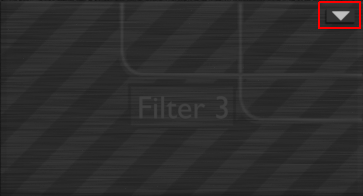
\includegraphics[width=0.5\textwidth]{graphics/filter_dropdown.png}
    \end{center}
}

\section{Common Controls}
Some of the controls are shared among most filter modules:

\begin{center}
    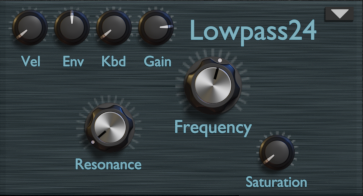
\includegraphics[width=0.5\textwidth]{graphics/lowpass_filter.png}
\end{center}

\audioparameter{Filter Frequency}{1}{1}
{Controls the cutoff point of the filter. The frequency value marks the point where the frequency is attenuated by 3dB.

    \begin{center}
        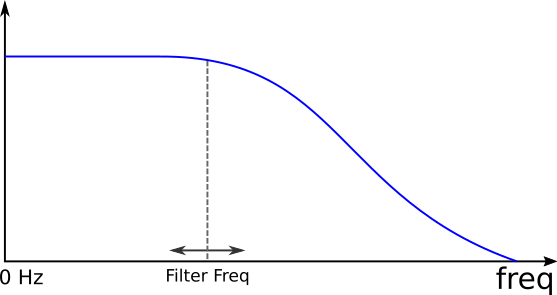
\includegraphics[width=0.5\textwidth]{graphics/filter_freq.png}
    \end{center}
}

\audioparameter{Filter Resonance}{1}{1}
{Increasing resonance creates a peak in the spectrum at the position of the filter cutoff.

    \begin{center}
        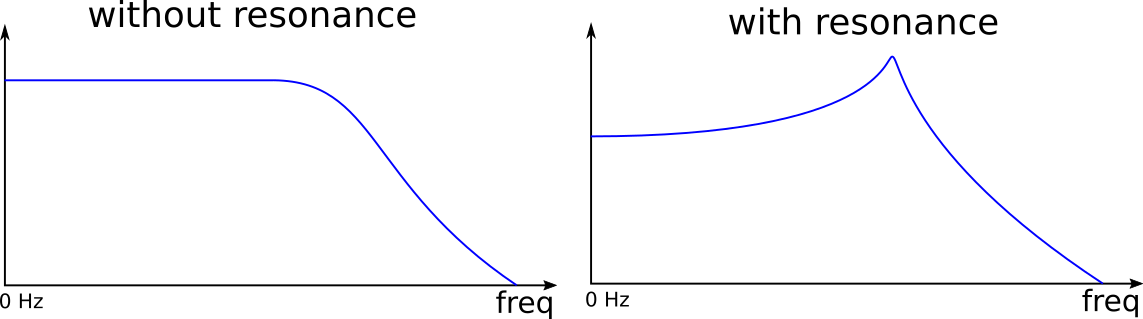
\includegraphics[width=0.9\textwidth]{graphics/filter_resonance.png}
    \end{center}

    Note also that the frequencies which were previously unaffected by the filter are being attenuated by the resonance parameter.

    None of the filters in Odin 2 are capable of self-oscillation for the sake of your ears and speakers.}

\audioparameter{Filter Velocity (Vel)}{1}{1}
{Adds velocity from MIDI-Notes to the filter frequency. This allows for expressive play, as harder key-hits move the filter freq up. Note that the value is added on top of the current value, so to achieve a similar resulting timbre, you might need to lower the filter frequency accordingly.}

\audioparameter{Filter Envelope (Env)}{1}{1}
{Controls the amount of Filter Envelope which is applied to the filter frequency. To see how the Filter Envelope itself is operated, see section \ref{ADSR}.}

\audioparameter{Filter Keyboard (Kbd)}{1}{1}
{Controls how much the MIDI-note is put on top of the filter frequency. Increasing this value makes the filter open up more for higher notes. This allows for more consistent notes across the keyboard, since higher notes might need higher filter freqs as well. Note that the value is added on top of the current value, so to achieve a similar resulting timbre, you might need to lower the filter frequency accordingly.}

\audioparameter{Filter Gain}{1}{1}
{Regulates the volume of this filter in deciBels. Can be used to shut the filter entirely. Modulating this parameter from the \modmatrix  with $-100$ will always shut the sound. Modulating this parameter with $+100$ will raise the sound to 0dB if the current value is smaller than -12dB. If it is bigger than -12dB, it will modulate to +12dB from the current value.}

\audioparameter{Filter Saturation}{1}{1}
{Introduces a slight distortion by shaping the signal with a hyperbolic tangent function. Depending on the filter module being used, the saturation stage is in a different position of the signal loop, yielding different results.}

\section{Lowpass, Bandpass, Highpass}
\begin{center}
    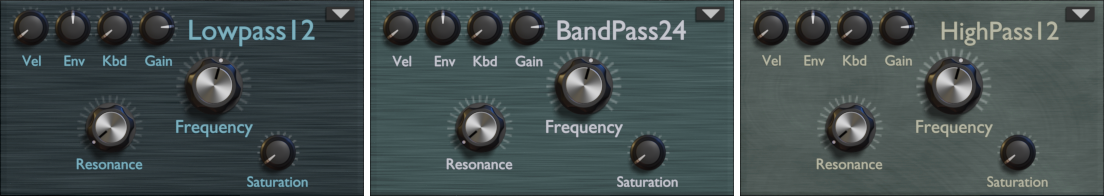
\includegraphics[width=\textwidth]{graphics/lp_bp_hp.png}
\end{center}

The staples of sound-design in Odin 2. These filters are virtual analog emulations of a certain, famous \fat{ladder filter} which has had a big impact in the history of synthesizers.

Each of these filters is available in a 12dB/Oct and a 24dB/Oct variant. These values determine the slope of the filter roll-off. The 24dB/Oct variants filter more frequencies than the 12dB/Oct counterparts.

\section{SEM-12}
\begin{center}
    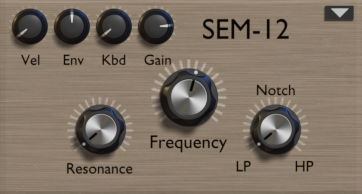
\includegraphics[width=0.5\textwidth]{graphics/SEM_filter.png}
\end{center}

Another emulation of a classic synthesizer filter. This filter has the specialty of being able to shift between a lowpass and a highpass filter, with a notch-filter in between. The filter slope of this filter is 12dB/Oct.

\audioparameter{SEM Transition}{1}{1}
{Fades from a lowpass filter over a notch filter to a highpass filter. This allows for special filter variants which still leave some of the frequencies that were filtered before.

    \begin{center}
        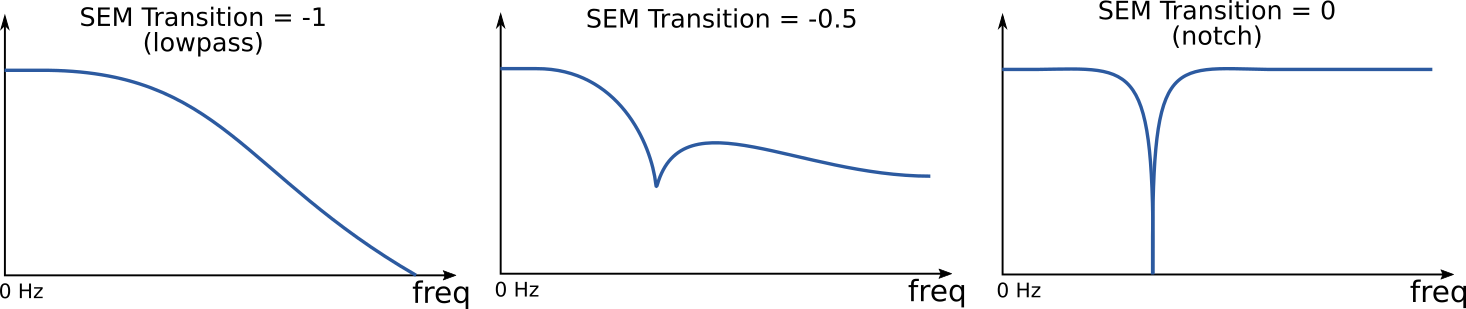
\includegraphics[width=\textwidth]{graphics/SEM_transition.png}
    \end{center}
}

\section{Diode Ladder}
\begin{center}
    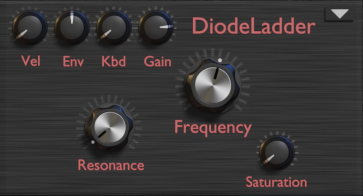
\includegraphics[width=0.5\textwidth]{graphics/diode_filter.png}
\end{center}

The Diode Ladder is a virtual analog emulation of another classic analog synthesizer filter. Its analog pendant was originally developed to work around a patent on the well established ladder filter. While still being 24dB/Oct, the characteristic of this filter is said to be more aggressive and wild compared to the classic ladder, especially when invoking resonance.

\section{KRG-35 LP / HP}
\begin{center}
    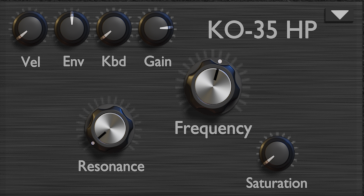
\includegraphics[width=0.5\textwidth]{graphics/korg_filter.png}
\end{center}

Yet another virtual analog emulation of one of the legendary analog filters of the past. This filter comes in a lowpass and highpass variant. Cranking up the resonance on these filters reveals a dirty, aggressive sound. Note that while the filters are named KRG-35, their slope is 12dB/Oct.

\section{Comb Filter}
\label{comb_filter}
\begin{center}
    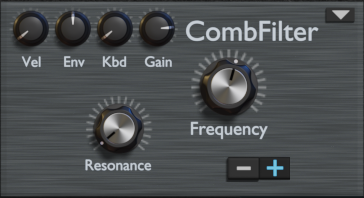
\includegraphics[width=0.5\textwidth]{graphics/comb_filter.png}
\end{center}

A comb filter is essentially a tuned \hyperref[delay]{delay module}. The input signal fed into a delay-line, which echos the sound back after a set amount of time. The delay time is the inverse of the filter frequency:

\begin{equation}
    t_{delay} = \frac{1}{f_{freq}}
\end{equation}

The frequency response of this filter usually resembles the shape of a hair-comb, hence the name.
\begin{center}
    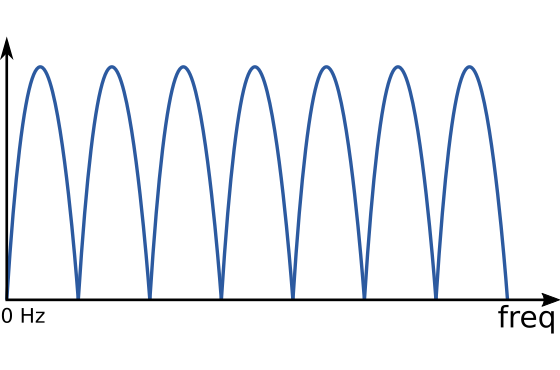
\includegraphics[width=0.5\textwidth]{graphics/comb_response.png}
\end{center}

The resonance parameter for the Comb Filter controls how much of the delayed signal is fed back into the delay line again, creating a feedback loop.

Comb filters can sound from subtle to metallic. When automating or modulating the frequency with high resonance values, a psychedelic smearing effect can be produced.

\audioparameter{Comb Polarity (+/-)}{0}{1}{
    Controls whether the insertion of the signal into the delay line is positive (+) or inverted (-). This changes the frequency behaviour. Inverted operation tends to eliminate deep frequencies.
}

\section{Formant Filter}
\begin{center}
    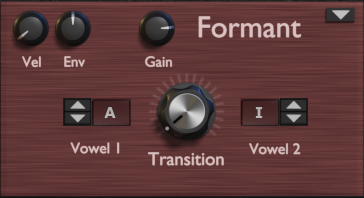
\includegraphics[width=0.5\textwidth]{graphics/formant_filter.png}
\end{center}
The Formant Filter tries to emulate vowels as they are produced in human speech. A tone is perceived as a vowel if two characteristic frequencies are dominant. These are called formants. The Formant Filter emulates this by using a combination of two resonator filters, which increase the frequencies around the two formants.

\begin{center}
    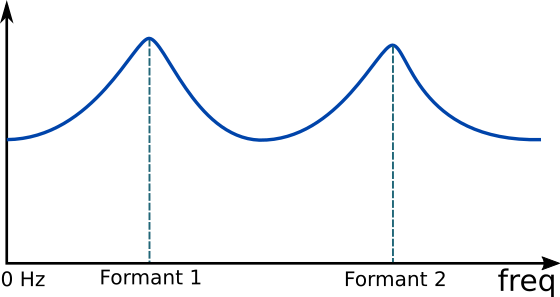
\includegraphics[width=0.5\textwidth]{graphics/formant_response.png}
\end{center}

The Formant Filter allows you to choose two vowels and freely move the formant peaks between the according formant peaks.

\audioparameter{Vowel 1 \& 2}{0}{0}{
    Select the vowels to the left and right of the transition. Selectable vowels are:

    A, E, I, O, U, \"A, \"O, \"U
}

\audioparameter{Formant Transition}{1}{1}{
    Transition between the two selected vowels. The transition is not a simple interpolation of the two vowel sounds, but actually moves the resonant formant peaks in the spectrum from one vowel to the next.

    The parameters Filter Velocity and Filter Envelope are applied to this parameter for the formant filter.
}

\section{Ring Modulator}
\begin{center}
    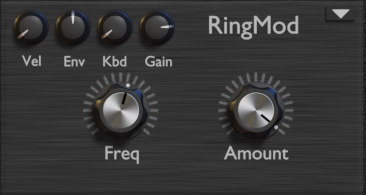
\includegraphics[width=0.5\textwidth]{graphics/ring_modulator.png}
\end{center}
The ring modulator is an oscillator disguised as a filter. The function of this module is to multiply the input signal with an internal sine-oscillator. This is formerly known as amplitude modulation.

\audioparameter{RingMod Freq}{1}{1}{
    Controls the frequency of the internal oscillator.
}

\audioparameter{RingMod Amount}{1}{1}{
    Controls the amount of ringmod to be applied. This interpolates between the input signal and the processed signal, effectively working like a Dry/Wet control.
}

